\section{Building Block View}\label{sec:building-block-view}

\subsection{Level 1}\label{subsec:level-1}

The high-level architecture provides a comprehensive overview of the main components and their interactions within the system, as depicted in Figure~\ref{fig:system_overview}.
The architecture comprises a frontend, a backend service, a database, and the Microsoft OAuth 2.0 authentication service.

\begin{figure}[ht]
    \centering
    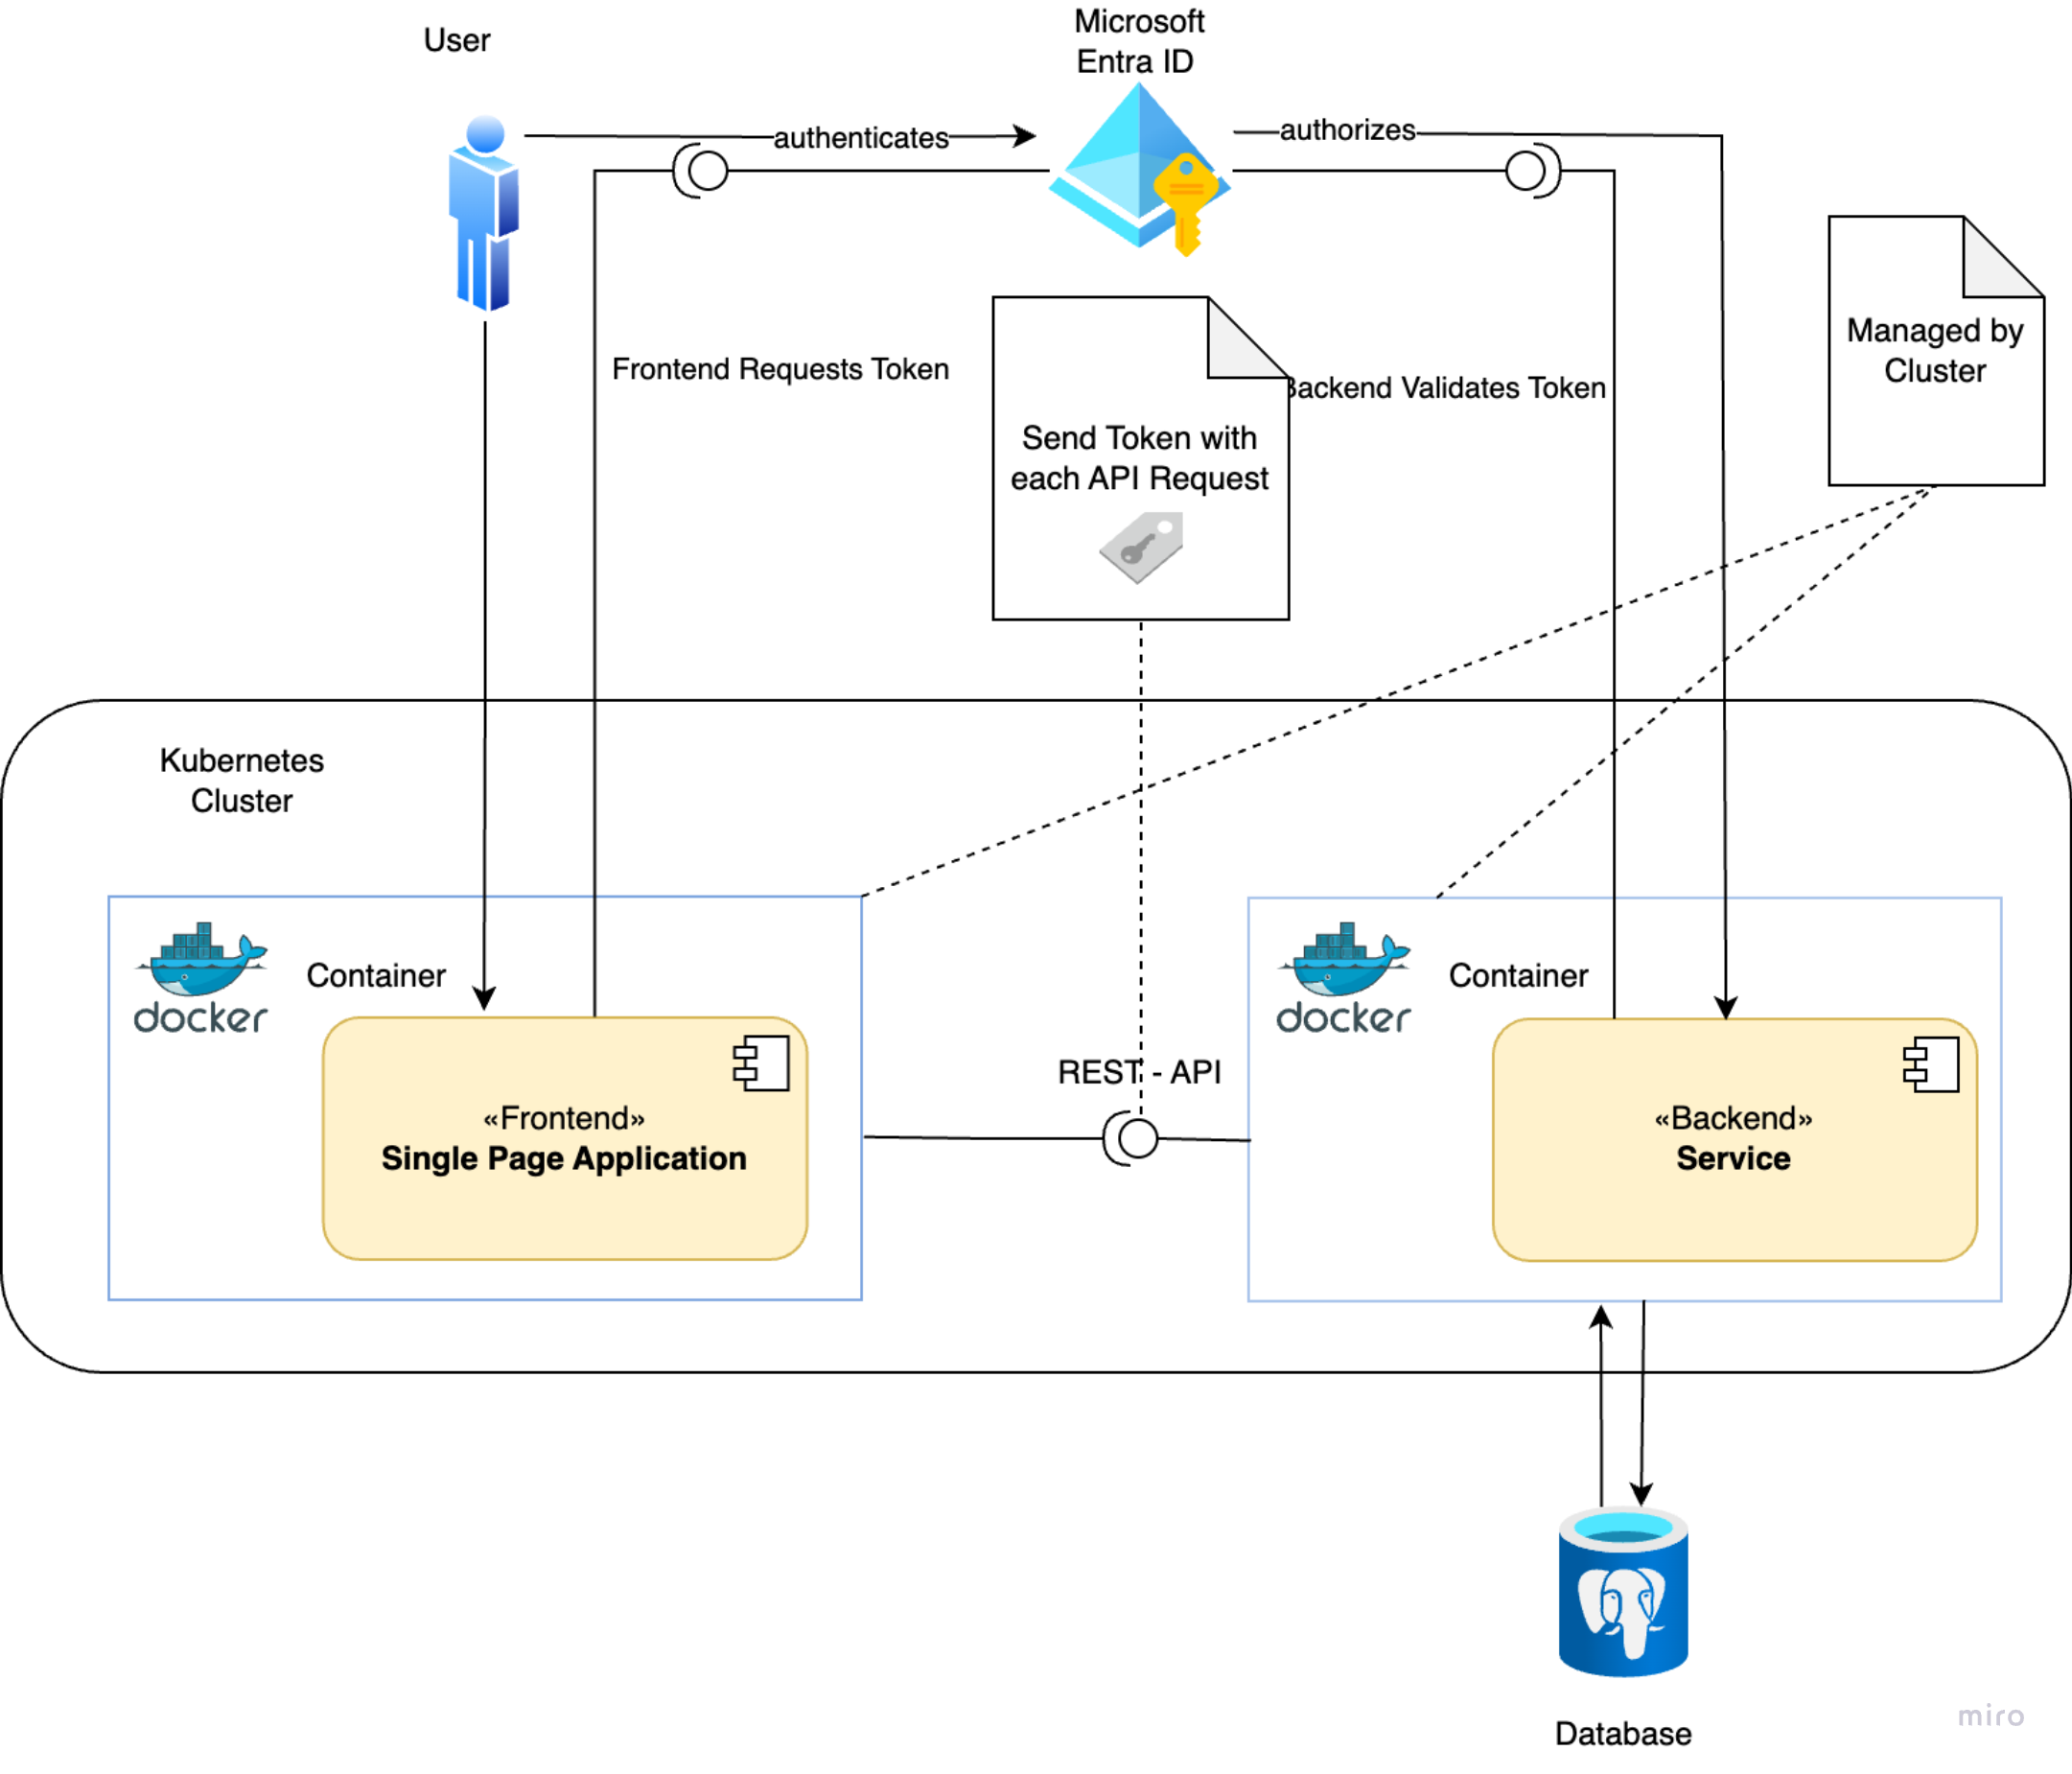
\includegraphics[width=\textwidth]{./images/high_level_architecture/system_overview}
    \caption{System Overview of the High-Level Architecture}
    \label{fig:system_overview}
\end{figure}

Users interact with the application through a Single Page Application (SPA) built with Angular.
This SPA frontend communicates with the backend service through a RESTful API that facilitates CRUD operations (Create, Read, Update, Delete) based on user-provided data.
For every request, an authentication token is utilized, provided by the Microsoft OAuth 2.0 service and validated with the backend service.

The backend component, developed in Golang, manages business logic processing and interacts directly with the PostgreSQL database to persistently store and retrieve the required data.

Both the frontend and the backend are hosted in Docker containers and orchestrated by a Kubernetes cluster, which ensures a scalable and manageable infrastructure.
This setup promotes efficient resource utilization and simplifies the deployment and management of the application.

The security of the system is bolstered by employing OAuth 2.0 for authentication and secure token transmission with API requests.
The RESTful API ensures a clear separation between the frontend and backend, enhancing the maintainability and extensibility of the system.

Highlighted Advantages:\\

\begin{itemize}
    \item \textbf{Scalability:} The use of Kubernetes for container orchestration allows the system to handle increasing loads efficiently, making it well-suited for dynamic scaling.
    \item \textbf{Security:} OAuth 2.0 integration provides a robust authentication mechanism, ensuring secure access control and token management.
    \item \textbf{Maintainability:} With a clear separation of concerns facilitated by the RESTful API, the system offers enhanced maintainability, allowing for independent updates and evolution of the frontend and backend.
    \item \textbf{Resource Optimization:} Containerization with Docker leads to optimized resource usage, as it enables lightweight and consistent deployments across various environments.
    \item \textbf{Developer Experience:} The adoption of popular frameworks like Angular for the frontend and Golang for the backend offers a productive environment for developers with strong community support and streamlined development workflows.
\end{itemize}

\subsubsection{Interaction with External Systems}\label{subsubsec:interaction-with-external-systems}

The application's ability to interact with external systems is a pivotal aspect of its design, offering both flexibility and extended functionality. A critical external system interaction is with the Microsoft OAuth 2.0 service, which provides user authentication and authorization capabilities.

\paragraph{Authentication with OAuth 2.0}
When a user attempts to access the application, the frontend initiates the authentication flow by redirecting the user to the Microsoft OAuth 2.0 service. The user then authenticates using their Microsoft credentials. Upon successful authentication, the service issues an access token and redirects the user back to the application.

The access token represents the user's identity and permissions, which the application can use to ensure that the user can only perform actions they are authorized for. This token is then included in the HTTP Authorization header in each subsequent API request made by the SPA to the backend.

\paragraph{Backend Token Validation}
Upon receiving an API request, the backend service extracts the token from the Authorization header and performs validation checks. While the token is issued by the OAuth service, the backend service needs to verify its integrity and validity. This is done by:

\begin{itemize}
    \item Ensuring the token is not expired.
    \item Verifying the token's signature to confirm that the issuer is the trusted OAuth 2.0 service.
    \item Checking the token's scopes to determine if the user is authorized to perform the requested action.
\end{itemize}

The backend service may occasionally need to communicate with the OAuth 2.0 service for tasks such as token introspection or revocation, especially when implementing log out functionality or for enhanced security checks.

\paragraph{Advantages of OAuth 2.0 Integration}
The integration with the OAuth 2.0 service offers several benefits:
\begin{itemize}
    \item \textbf{Delegated Authentication:} The system leverages the robust, secure authentication mechanisms provided by Microsoft, thus delegating the authentication responsibility and reducing the system's attack surface.
    \item \textbf{Single Sign-On (SSO):} Users benefit from a seamless experience by using a single set of credentials across multiple applications within the Microsoft ecosystem.
    \item \textbf{Access Control:} The OAuth 2.0 service effectively manages access control, ensuring that users can only access resources for which they have been granted permissions.
    \item \textbf{Reduced Complexity:} The backend does not need to handle user credentials directly, simplifying the security model and reducing the complexity of the backend service.
\end{itemize}

This interaction with external systems underscores the application's commitment to secure, efficient, and user-friendly operations, adhering to modern security practices and standards.

\subsection{Level 2}\label{subsec:level-2}

\subsubsection{Detailed View of Database}

The database structure is crucial for understanding the persistence layer of the application.
The following subsections outline the database schema, defined by SQL tables, and the relationships between them, as represented in the Entity-Relationship (ER) Diagram.

\headingThree{User Table}
The \texttt{user} table stores information about users, uniquely identified by an internal ID and an OAuth identifier which enables authentication through external services like Microsoft Entra ID. The table ensures the application's flexibility to adapt to different authentication methods without altering the core data model.

\headingThree{Project Table}
The \texttt{project} table captures details of various projects within the system.
Each project has a unique name, a description, and a timestamp marking its creation.
This table is the cornerstone for grouping related items and extensions within the application.

\headingThree{Extension Table}
Extensions, defined in the \texttt{extension} table, can be optionally associated with a project, indicated by the  \texttt{project\_id} foreign key, allowing for shared or project-specific extensions.
The table also includes a scope attribute, name, description, and the creation timestamp.

\headingThree{Item Table}
The \texttt{item} table holds records of items, each associated with an extension and characterized by a unique name, type code, and storage table name.
This table is essential for tracking and managing individual items.

\headingThree{Role Assignment Table}
Role assignments are managed in the \texttt{role\_assignment} table, linking users to projects with assigned roles.
This table is pivotal for implementing access control within the system.

\headingThree{Indexes}
Indexes are suggested for frequently queried columns to optimize the database's performance.
These indexes, however, are commented out in the script and can be created as needed based on the application's query patterns.

\headingThree{ER Diagram}
Figure~\ref{fig:er_diagram} presents the Entity-Relationship (ER) Diagram, visualizing the tables and their relationships, reflecting the described schema.

\begin{figure}[H]
    \centering
    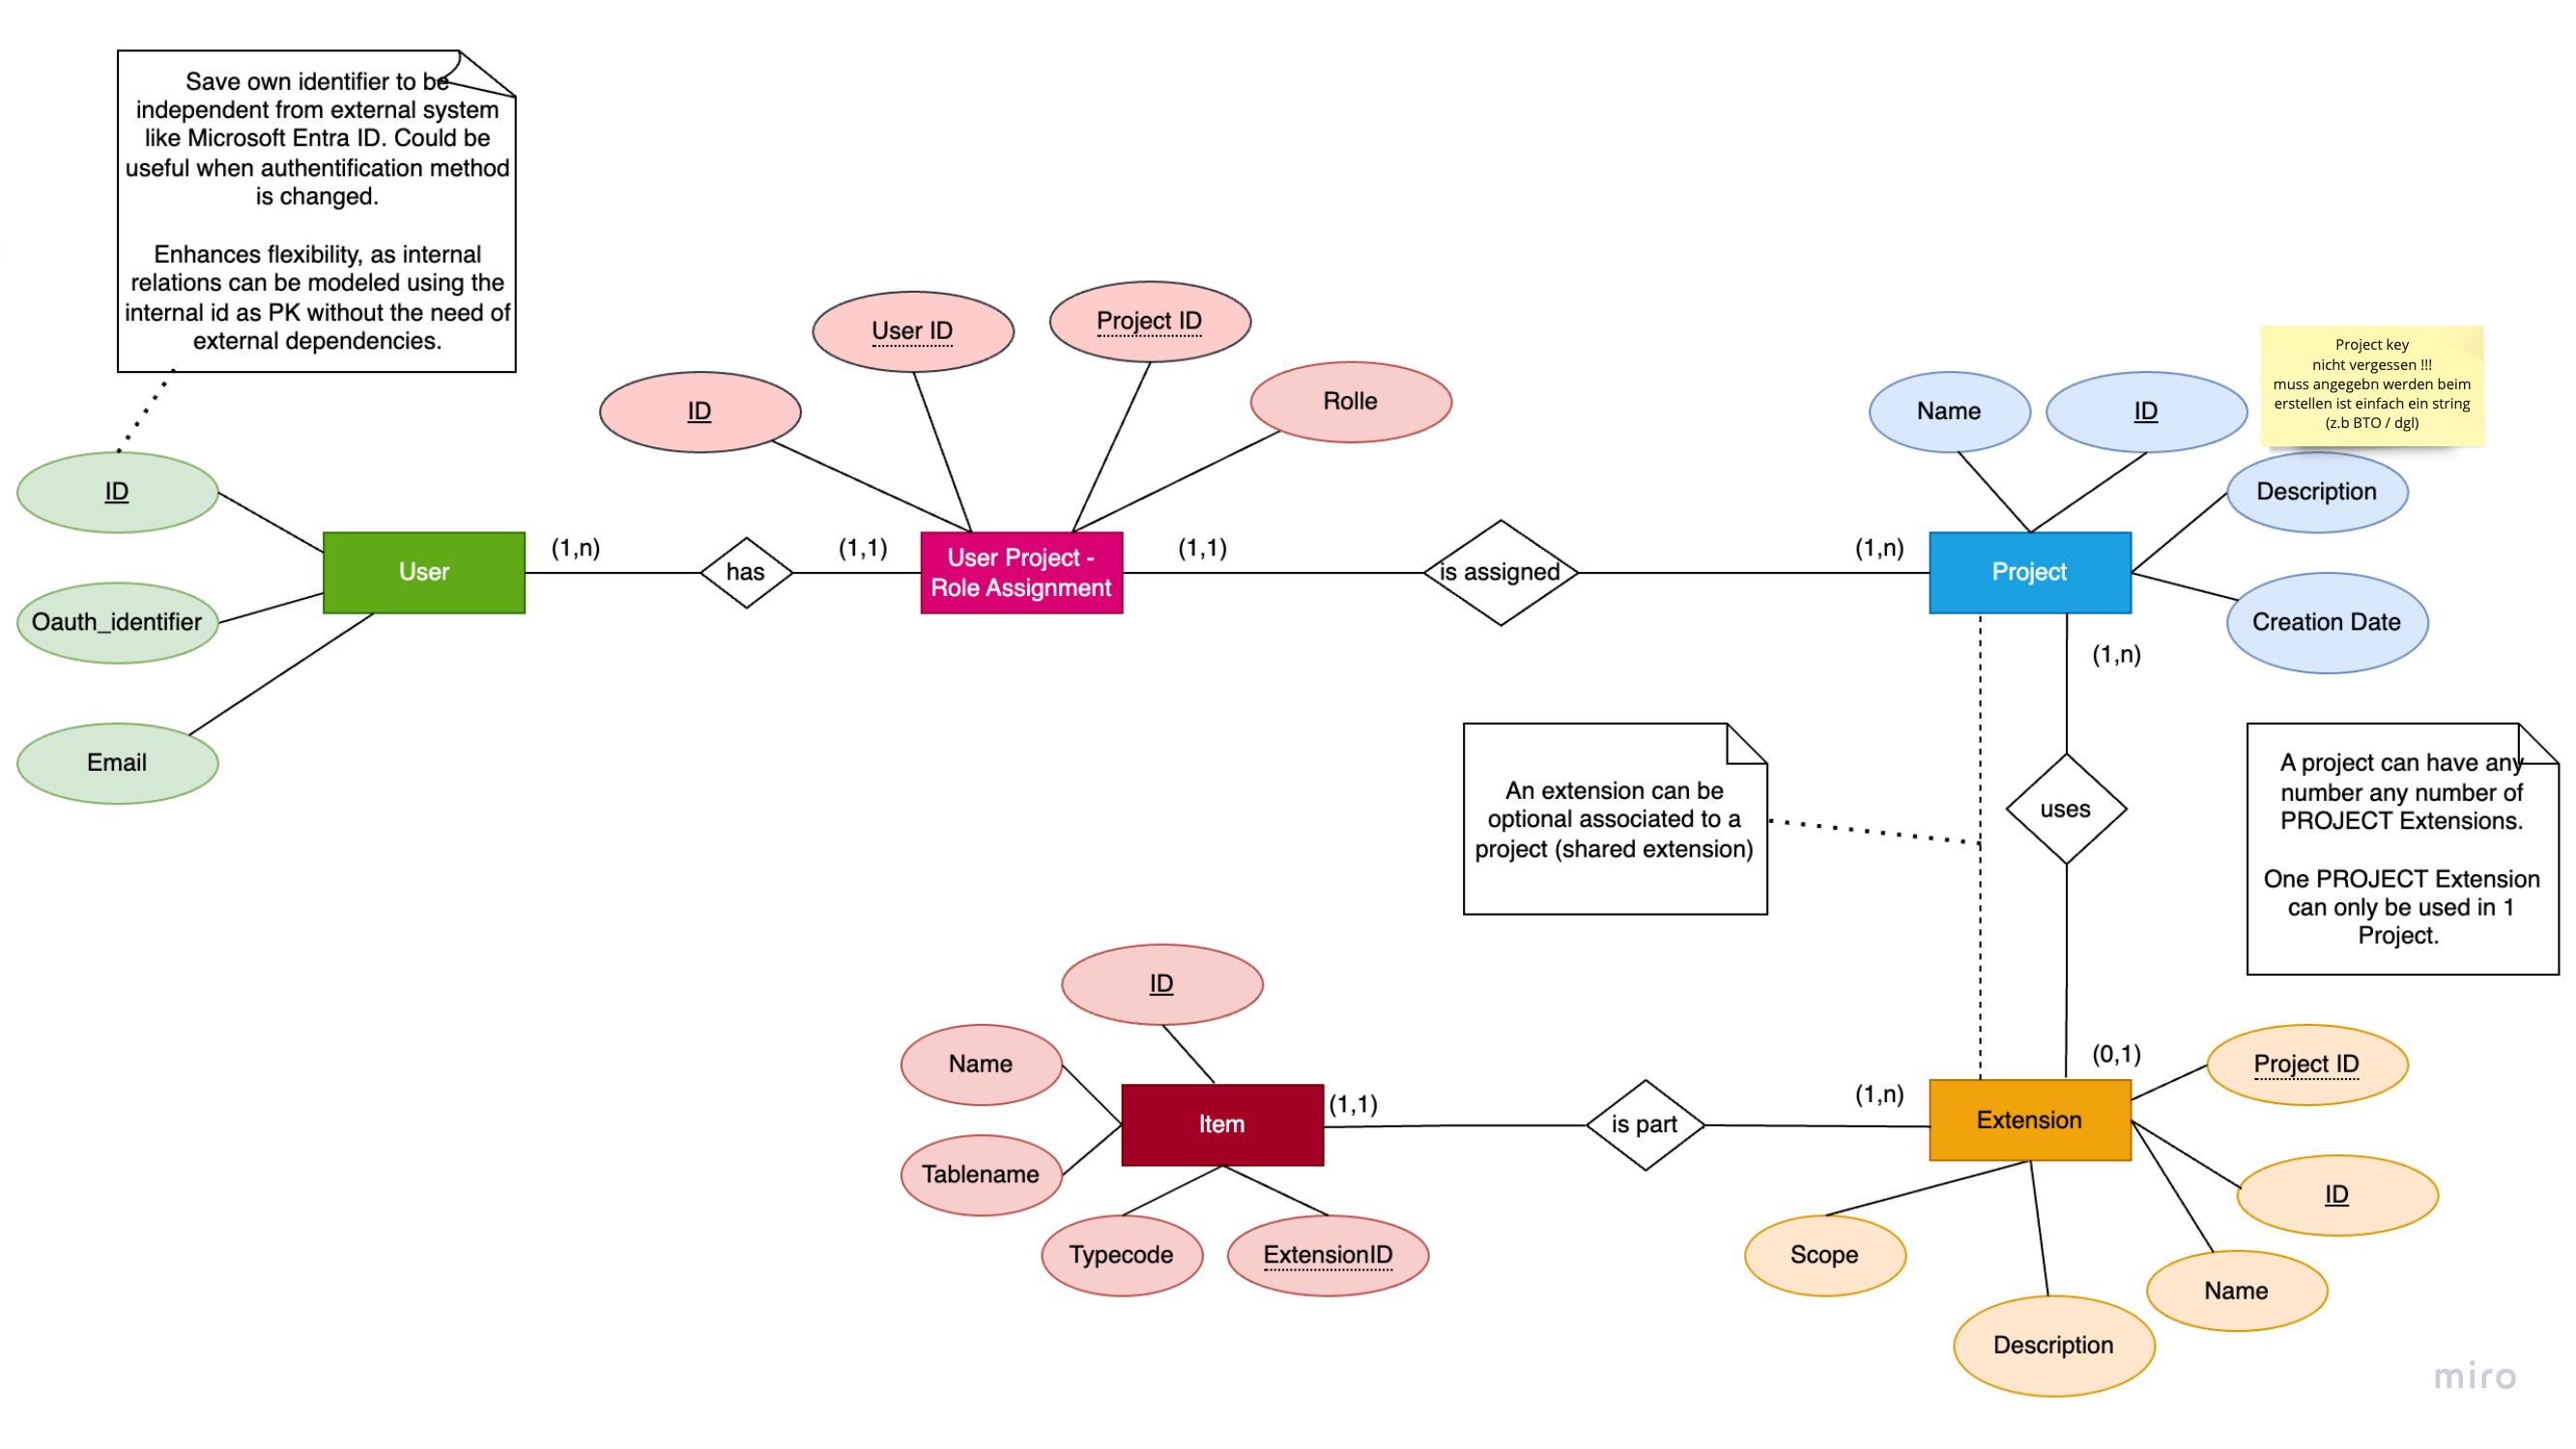
\includegraphics[width=\textwidth]{./images/database/er_diagram}
    \caption{Entity-Relationship Diagram of the Database}
    \label{fig:er_diagram}
\end{figure}


Furthermore, constraints and indexes are crucial aspects of the design and should be enabled based on the database performance requirements and query analysis.

\subsubsection{Detailed View of Backend}
The backend system serves as the backbone of our application, orchestrating the core logic, data management, and security protocols.
Developed in Golang, it interfaces seamlessly with the Angular-based frontend by providing a robust RESTful API. This API facilitates CRUD (Create, Read, Update, Delete) operations, essential for managing the application's data effectively.
Furthermore, the backend is responsible for authenticating users via the Microsoft OAuth 2.0 service, ensuring secure access to the application's features.
It also interacts directly with the PostgreSQL database, handling data persistence and retrieval, thus maintaining the integrity and consistency of the application state across multiple user sessions.

The backend architecture is visualized in Figure~\ref{fig:backend_architecture} below, providing a schematic overview of the main modules and their interactions.

\begin{figure}[ht]
    \centering
    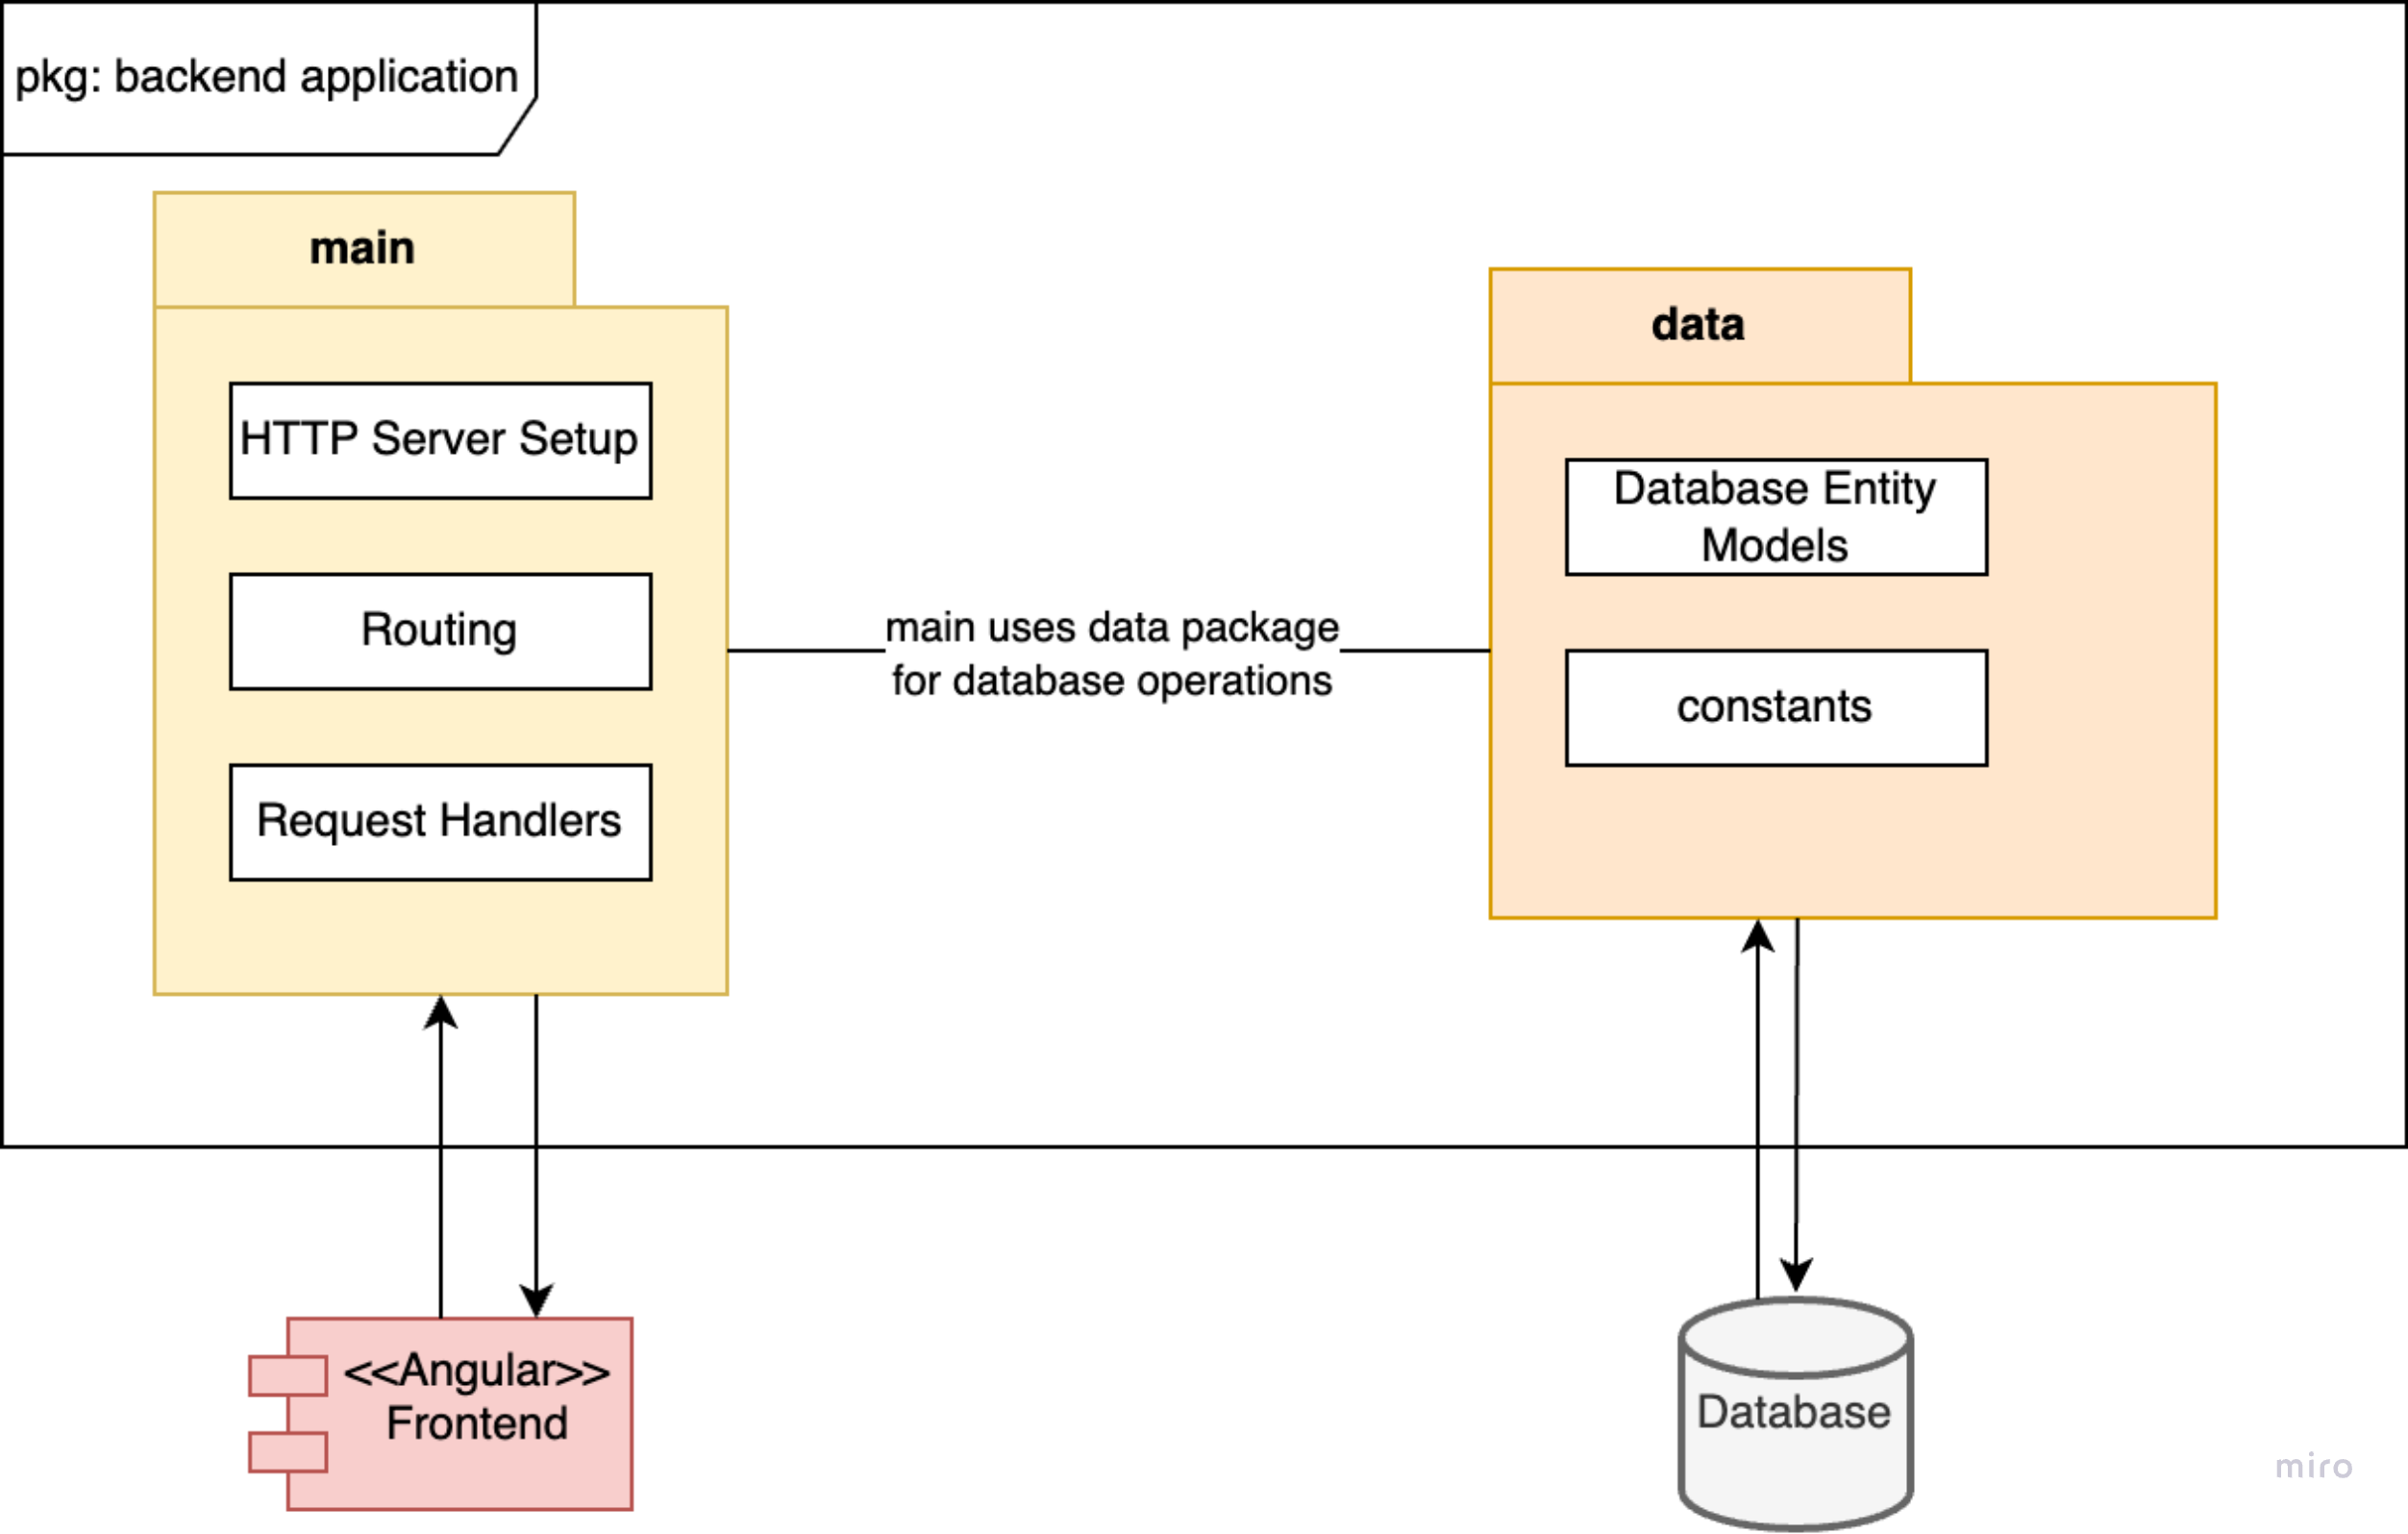
\includegraphics[width=\textwidth]{images/backend/backend_pkg_level_2}
    \caption{Schematic overview of the backend architecture}
    \label{fig:backend_architecture}
\end{figure}

\headingFour{Packages and Libraries}
The backend's technology stack is meticulously chosen to leverage the robustness and simplicity offered by Golang, aligning with our objectives for performance, scalability, and maintainability. Key aspects of our technology stack include:

\begin{itemize}
    \item \textbf{HTTP Routing:} Instead of third-party libraries, we utilize Golang's standard `http` package for routing, taking advantage of its powerful and efficient HTTP server capabilities. This approach allows for direct control over route handling and middleware integration, ensuring optimal performance and compatibility with Go's native paradigms.

    \item \textbf{Database Interaction:} For database connectivity and operations, we rely on the standard `database/sql` package.
    This choice provides a lightweight, flexible interface to our PostgreSQL database, enabling efficient management of connections and the execution of SQL queries.

    \item \textbf{Entity Management:} Each data entity, such as `Item`, is defined within its package, encapsulating the CRUD operations.
    This pattern ensures a clear separation of concerns and enhances the maintainability of our data access layer.
    By implementing entity-specific types and methods, we gain fine-grained control over database interactions, allowing for customized query optimization and error handling strategies.

    \item \textbf{Logging:} `zerolog` package is used as a logging framework.
    It brings structured, level-based logging, which is highly performant and customizable.
    With `zerolog`, log messages can be defined at various levels, from `trace` to `fatal`, providing clear visibility into the application's behavior and aiding in prompt issue resolution.
\end{itemize}

This technology stack, grounded in Golang's standard libraries and best practices, forms the backbone of our backend architecture.
It enables us to build a system that is not only performant and reliable but also cohesive with Go's design philosophy, ensuring ease of development and future scalability.

\headingFour{Routing and HTTP Handling}
Our backend leverages the standard `http` package from Golang's standard library for routing and HTTP request handling.
This approach allows us to directly use the powerful concurrency features of Go without the need for external frameworks, keeping the application lightweight and efficient.

\begin{longtable}{|l|p{3cm}|>{\raggedright\arraybackslash}p{7cm}|}
    \hline
    \rowcolor{headercolor} \textbf{Route} & \textbf{Methods} & \textbf{Description} \\
    \endfirsthead

    \hline
    \rowcolor{headercolor} \textbf{Route} & \textbf{Methods} & \textbf{Description} \\
    \endhead

    \hline
    /healthcheck & GET & This route returns the current state of the API and can be used to retrieve status information. \\
    \hline
    /items & GET, POST & This route fetches all items or creates a new item.
    In the POST request body, the client needs to send the following data:
    \newline\newline  - \textbf{name}: A string representing the name of the item to create.
    \newline\newline - \textbf{tablename}: A string representing the name of the table holding item entries in SAP.
    \newline\newline - \textbf{extension\_id}: A number representing the unique identifier of an existing extension. Depending on the id, the backend determines if the item will be created for a global or project scope (depending on the scope of the extension). \\
    \hline
    /items/ & GET, PUT, DELETE & Gets, updates, or deletes an item by its ID. Updating an item is idempotent \\
    \hline
    /projects & GET & Returns all projects created. \\
    \hline
    /extensions & GET & Returns all extensions created). \\
    \hline
    /extensions/ & GET & Gets the extensions of a specific scope.
    Only two values will return extensions:
    \newline\newline - \textbf{Shared}: Returns all the shared extensions.
    \newline\newline - \textbf{Project}: Returns all Project extensions. \\
    \hline
    \caption{Overview of Backend Routes}
    \label{tab:table_routes}
\end{longtable}

\headingFive{API Examples}\label{subsubsec:api-examples}

In this section, we provide examples of API calls and their corresponding responses.
These examples illustrate how clients interact with our API.

\headingSix{GET /healthcheck}

This API endpoint is used to check the health of the service.

\begin{lstlisting}[language=json,label={lst:lstlisting6}]
GET /healthcheck HTTP/1.1
Host: example.com
\end{lstlisting}

Response:

\begin{lstlisting}[language=json,label={lst:lstlisting4}]
HTTP/1.1 200 OK
Content-Type: application/json

{
    "status": "OK"
}
\end{lstlisting}

\headingSix{GET /items}

The \texttt{GET /items} endpoint provides clients with the ability to retrieve a list of all items in the system.
When a client makes a \texttt{GET} request to the \texttt{/items} endpoint, the backend service will return a list of all items.
If there are no items in the system, the server will respond with a \texttt{200 OK} status code and an empty list.

\begin{lstlisting}[language=json,label={lst:lstlisting3}]
GET /items HTTP/1.1
Host: example.com
\end{lstlisting}

Response:

\begin{lstlisting}[language=json,label={lst:lstlisting}]
HTTP/1.1 200 OK
Content-Type: application/json

{
    "items": [
        {
            "id": 31,
            "scope": "Project",
            "project": "Projekt A",
            "name": "New Item",
            "table_name": "new_table",
            "extension_id": 1,
            "typecode": 14010,
            "creation_date": "2024-04-27T09:11:53.584653Z"
        },
        {
            "id": 30,
            "scope": "Project",
            "project": "Projekt A",
            "name": "New Item",
            "table_name": "new_table",
            "extension_id": 1,
            "typecode": 14009,
            "creation_date": "2024-04-27T09:09:59.94747Z"

        }
    ]
}
\end{lstlisting}

\headingSix{POST /items}

When a client makes a \texttt{POST} request to the \texttt{/items} endpoint, they must include a JSON object in the request body.
This object should contain the following fields:

\begin{itemize}
    \item \texttt{name}: A string representing the name of the item to be created.
    \item \texttt{table\_name}: A string representing the name of the table which will then hold the newly created item entries in SAP.
    \item \texttt{extension\_id}: A number representing the unique identifier of an existing extension.
    Depending on the id, the backend determines if the item will be created for a global or project scope (depending on the scope of the extension).
\end{itemize}

Upon receiving a valid \texttt{POST} request, the backend service will create a new item with the provided details.
It will then return a \texttt{201 Created} status code along with a JSON object containing the details of the newly created item.

\begin{lstlisting}[language=json,label={lst:lstlisting7}]
POST /items HTTP/1.1
Host: example.com
Content-Type: application/json

{
    "name": "New Item",
    "table_name": "new_table",
    "extension_id": 1
}
\end{lstlisting}

Response:

\begin{lstlisting}[language=json,label={lst:lstlisting8}]
HTTP/1.1 201 Created
Content-Type: application/json

{
    "id": 34,
    "scope": "Project",
    "project": "",
    "name": "New Item",
    "table_name": "new_table",
    "extension_id": 1,
    "typecode": 14011,
    "creation_date": "2024-04-27T19:13:22.781434Z"
}
\end{lstlisting}

\headingSix{GET /items/{id}}

The \texttt{GET /items/\{id\}} endpoint allows clients to retrieve a specific item by its unique identifier.
When a client makes a \texttt{GET} request to the \texttt{/items/\{id\}} endpoint, the backend service will return the details of the item with the provided ID. If an item with the given ID does not exist, the server will respond with a \texttt{404 Not Found} status code.

\begin{lstlisting}[language=json,label={lst:lstlisting9}]
GET /items/1 HTTP/1.1
Host: example.com
\end{lstlisting}

Response:

\begin{lstlisting}[language=json,label={lst:lstlisting10}]
HTTP/1.1 200 OK
Content-Type: application/json

{
    "id": 1,
    "scope": "Project",
    "project": "Project A",
    "name": "Item A1",
    "table_name": "Table A1",
    "extension_id": 1,
    "typecode": 14000,
    "creation_date": "2024-04-24T20:02:00.573142Z"

}
\end{lstlisting}

\headingSix{Delete /items/{id}}

When a client makes a \texttt{DELETE} request to the \texttt{/items/{id}} endpoint, they must provide the ID of the item they want to delete in the endpoint URL.
Upon receiving a valid \texttt{DELETE} request, the backend service will attempt to delete the item with the provided ID.
If the item exists and is successfully deleted, the service will return a \texttt{200 OK} status code, indicating that the request was successful.

\begin{lstlisting}[language=json,label={lst:lstlisting7}]
DELETE /items/3 HTTP/1.1
Host: example.com
\end{lstlisting}

Response:

\begin{lstlisting}[language=json,label={lst:lstlisting8}]
HTTP/1.1 204 No Content
\end{lstlisting}

\headingSix{PUT /items/{id}}

When a client makes a \texttt{PUT} request to the \texttt{/items/{id}} endpoint, they must provide the ID of the item they want to update in the endpoint URL.)
In the request body, the client must include a JSON object with the updated details of the item.
The following values can be updated:
\begin{itemize}
    \item \texttt{name}: A string representing the name of the item.
    \item \texttt{table\_name}: A string representing the name of the table which will then hold the item entries in SAP.
\end{itemize}

Upon receiving a valid \texttt{PUT} request, the backend service will attempt to update the item with the provided ID.
If the item exists and is successfully updated, the service will return a \texttt{204 NoContent} status code to indicate that the request was successful.

\begin{mynote}
    NOTE: The following fields can not be updated: \\ \texttt{scope}, \texttt{project}, \texttt{extension\_id}, \texttt{typecode}, \texttt{creation\_date}.
    Changing these fields would require more complex operations and is not supported by this endpoint, as changing the typecode would require changing the item's scope for example.
    Changing the scope would require moving the item to a different extension, which is not supported by this endpoint.
\end{mynote}

\begin{lstlisting}[language=json,label={lst:lstlisting21}]
PUT /items/1 HTTP/1.1
Host: example.com

{
    "name": "New Name",
    "table_name": "New Table Name",
}

\end{lstlisting}

\headingSix{GET /projects}

The \texttt{GET /projects} endpoint allows clients to retrieve all projects in the system.
When a client makes a \texttt{GET} request to the \texttt{/projects} endpoint, the backend service will return a list of all projects.
\\Each project in the list includes details such as the project's `id`, `name`, `description`, and `creation\_date`.

\begin{lstlisting}[language=json,label={lst:lstlisting11}]
GET /projects HTTP/1.1
Host: example.com
\end{lstlisting}

Response:

\begin{lstlisting}[language=json,label={lst:lstlisting12}]
HTTP/1.1 200 OK
Content-Type: application/json

{
    "projects": [
        {
            "id": 1,
            "name": "Project 1",
            "description": "This is project 1",
            "creation_date": "2023-01-01T00:00:00Z"
        },
        {
            "id": 2,
            "name": "Project 2",
            "description": "This is project 2",
            "creation_date": "2023-01-02T00:00:00Z"
        }
    ]
}
\end{lstlisting}

\headingSix{GET /extensions}

The \texttt{GET /extensions} endpoint allows clients to retrieve all extensions in the system.
When a client makes a \texttt{GET} request to the \texttt{/extensions} endpoint, the backend service will return a list of extensions.

\begin{lstlisting}[language=json,label={lst:lstlisting13}]
GET /extensions HTTP/1.1
Host: example.com
\end{lstlisting}

Response:

\begin{lstlisting}[language=json,label={lst:lstlisting23}]
HTTP/1.1 200 OK
Content-Type: application/json

{
    "extensions": [
        {
            "id": 1,
            "project_id": null,
            "name": "Extension 1",
            "description": "This is extension 1",
            "scope": "Shared",
            "creation_date": "2023-01-01T00:00:00Z"
            "item_count: 2"
        },
        {
            "id": 2,
            "project_id": 2,
            "name": "Extension 2",
            "description": "This is extension 2",
            "scope": "Project",
            "creation_date": "2023-01-02T00:00:00Z"
            "item_count: 10"
        }
    ]
}
\end{lstlisting}


\headingSix{GET /extensions/{scope}}
The client has the option to specify the scope of the extensions they want to retrieve.
Therefore, the client can include the scope consisting of either `shared` or `project` in the request URL\@.
The returned extensions are then filtered based on their scope, which can be either 'Shared' or 'Project'.
The 'Shared' scope returns all the shared extensions, while the 'Project' scope returns all project extensions.

\begin{lstlisting}[language=json,label={lst:lstlisting22}]
GET /extensions/project HTTP/1.1
Host: example.com
\end{lstlisting}

\begin{lstlisting}[language=json,label={lst:lstlisting14}]
HTTP/1.1 200 OK
Content-Type: application/json

{
    "extensions": [
        {
            "id": 1,
            "project_id": 1,
            "name": "Extension 1",
            "description": "This is extension 1",
            "scope": "Project",
            "creation_date": "2023-01-01T00:00:00Z"
            "item_count: 2"
        },
        {
            "id": 2,
            "project_id": 2,
            "name": "Extension 2",
            "description": "This is extension 2",
            "scope": "Project",
            "creation_date": "2023-01-02T00:00:00Z"
            "item_count: 0"
        }
    ]
}
\end{lstlisting}

\begin{itemize}
    \item \textbf{Health Check}: A simple endpoint to verify the backend service's health.
    \item \textbf{CRUD Operations}: Endpoints for managing items, including creating, reading, updating, and deleting entries.
    These are mapped to specific handler functions that encapsulate the business logic.
    \item \textbf{Extensions and Projects}: Specific endpoints designed to handle operations related to extensions and projects within the system.
\end{itemize}

\headingFour{Data Access Layer}
The core of our data management strategy is the effective use of Go's `database/sql` package, providing a solid foundation for executing SQL queries and interacting with our PostgreSQL database.

\headingFive{Entity Management}
For each entity in our system, we define a Go struct that mirrors the database schema and implements the CRUD operations.
This approach offers type safety and clear encapsulation of database logic.

\headingSix{Example: Item Model}
The `Item` struct represents an item entity, including fields like `ID`, `Name`, `TableName`, and `Typecode`.
The `ItemModel` struct wraps a database connection pool, offering methods such as `Insert` to add new items to the database.

\begin{lstlisting}[language=Go,label={lst:lstlisting17}]
type ItemModel struct {
	DB *sql.DB
}
\end{lstlisting}

\begin{lstlisting}[language=Go,label={lst:lstlisting2}]
type Item struct {
    ID           int64     `json:"id"`
    Name         string    `json:"name"`
    TableName    string    `json:"table_name"`
    Typecode     int32     `json:"typecode"`
    ExtensionID  int64     `json:"extension_id"`
    CreationDate time.Time `json:"creation_date"`
}
\end{lstlisting}

The above struct is a representation of the item entity in the database.
The following picture illustrates the item in the database and shows the mapping between the struct and the database table.

\begin{figure}[ht]
    \centering
    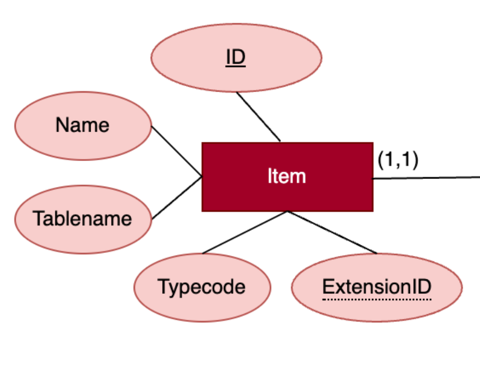
\includegraphics[scale=0.4]{./images/database/item_er}
    \caption{Item Entity in the Database}
    \label{fig:item_database_model}
\end{figure}

This pattern is replicated for other entities, ensuring consistent and organized data access throughout the application.

\headingFour{Logging with Zerolog}

The backend uses the `zerolog` library for its logging system.
`Zerolog` provides structured, level-based logging that is highly performant and scalable, making it suitable for both development and production environments.

\begin{itemize}
    \item \textbf{Log Levels:} Multiple log levels are available, enabling the appropriate granularity of log messages.
    These levels include:
    \begin{itemize}
        \item \textit{Trace}: The most verbose level, used for systematic granular events that are useful for debugging.
        \item \textit{Debug}: Used for less granular but still detailed debugging information about the system's behavior.
        \item \textit{Info}: Standard log level indicating general operational events that highlight the application's running state.
        \item \textit{Warn}: Indicates a potential issue or important event that should be noted but is not necessarily an error.
        \item \textit{Error}: Used when the application encounters an issue that disrupts a process or operation.
        \item \textit{Fatal}: Signifies a severe problem that has caused or is about to cause the application to terminate.
    \end{itemize}
    \item \textbf{Usage Context:} The backend strategically employs these log levels to enhance observability:
    \begin{itemize}
        \item \textit{Trace} and \textit{Debug} logs are predominantly used in development environments to trace execution flow and diagnose issues.
        \item \textit{Info} logs are recorded during routine operations, such as service start-up or shutdown, and when significant transactions occur.
        \item \textit{Warn} logs alert to conditions that require attention or may lead to an error if left unaddressed.
        \item \textit{Error} logs capture failures within the system, facilitating rapid diagnosis and resolution of issues.
        \item \textit{Fatal} logs are used sparingly, only logging critical events that will halt the backend services.
    \end{itemize}
\end{itemize}

By utilizing `zerolog`, the backend achieves efficient and structured logging, greatly improving the maintainability and performance of the system's logging capabilities.
With configurable output (console, JSON) and the ability to integrate with various logging platforms, `zerolog` enriches the operational monitoring and troubleshooting processes.


\newpage

\subsubsection{Detailed View of Frontend}
The frontend component of our application is a Single Page Application (SPA) developed using Angular.
This modern web framework offers a robust foundation for building interactive and responsive user interfaces, ensuring a seamless user experience.
The frontend interacts with the backend service through a RESTful API, enabling the application to perform CRUD operations on the data stored in the PostgreSQL database.

Figure~\ref{fig:frontend_architecture} provides a visual representation of the frontend architecture, outlining the main components and their interactions within the Angular application.

\begin{figure}[H]
    \centering
    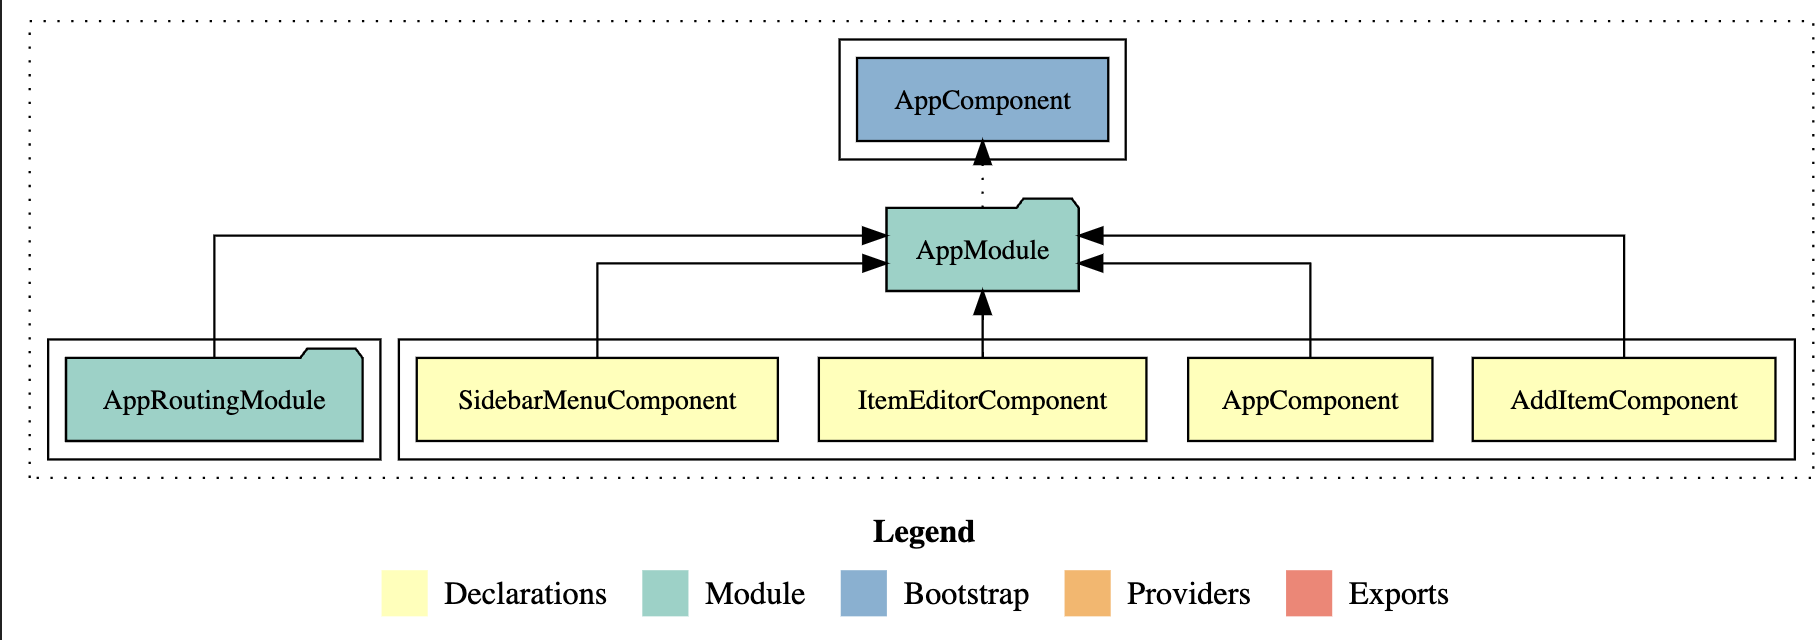
\includegraphics[width=\textwidth]{images/frontend/frontend_overview_component}
    \caption{Frontend architecture component diagram.}
    \label{fig:frontend_architecture}
\end{figure}

The \texttt{AppModule} serves as the root module of the Angular application, which bootstraps the \texttt{AppComponent} — the top-level component container.
Within \texttt{AppModule}, several feature components are declared, such as \\\texttt{HeaderComponent} and \texttt{ItemEditorComponent}.

The \texttt{ItemEditorComponent} is particularly interactive, featuring a button that, when clicked by the user, triggers the display of the \texttt{AddItemComponent}.
This component presents a form that users can use to input the details required to create a new item in the system.

Each component is designed to be a self-contained unit, managing its own display and behavior, thus promoting reusability and separation of concerns.
Services and shared modules are used to handle cross-cutting concerns such as data access and state management, further illustrated by their respective providers and exports within the diagram.

\headingFour{External Libraries and Dependencies}

\headingFive{Taiga UI}
Taiga UI is a modern Angular component library that provides a set of UI components and utilities to streamline frontend development.

Taiga UI is chosen for several reasons:

\begin{itemize}
    \item \textbf{Lightweight}: Taiga UI is designed to be lightweight, which can lead to faster load times and improved performance for your application.
    \item \textbf{Highly Customizable Themes}: Taiga UI provides a high level of theme customization. This allows developers to easily align the application's aesthetics with their company's branding or their specific design requirements.
    \item \textbf{Advanced Features}: Taiga UI comes with a set of advanced features out of the box, such as a built-in light and dark mode, multi-language support, and a focus management system.
    \item \textbf{Comprehensive Documentation}: Taiga UI has extensive and clear documentation, making it easier for developers to understand how to use and customize the components.
    \item \textbf{Active Community}: Taiga UI has an active community of developers. This means that if you encounter issues or need help, you're likely to get a response quickly.
    \item \textbf{Integration with Other Libraries}: Taiga UI can be easily integrated with other popular libraries such as ngRx, making it a flexible choice for many projects.
\end{itemize}

\headingFour{Documenting Angular Projects with Compodoc}

Compodoc is a powerful documentation tool specifically designed for Angular projects. It simplifies the process of documenting code, providing developers with comprehensive and easily navigable documentation.

\begin{itemize}
    \item \textbf{Features:} Compodoc offers a range of features to streamline the documentation process and improve project maintainability:
    \begin{itemize}
        \item \textit{Automatic Generation}: Compodoc automatically generates documentation from Angular projects, eliminating the need for manual documentation creation.
        \item \textit{Live Preview}: Developers can preview documentation changes in real-time, ensuring accuracy and consistency before finalizing the documentation.
        \item \textit{Code Visualization}: Compodoc visualizes the structure of Angular projects, including modules, components, directives, services, and more, making it easier to understand and navigate the codebase.
        \item \textit{Customization}: Developers can customize the appearance and content of the generated documentation, tailoring it to the specific needs of the project or team.
        \item \textit{Search and Navigation}: Compodoc provides powerful search and navigation capabilities, allowing users to quickly find relevant documentation and navigate between different parts of the codebase.
    \end{itemize}
    \item \textbf{Usage Context:} Compodoc is integrated into our Angular development workflow to enhance project documentation and collaboration:
    \begin{itemize}
        \item \textit{Developer Onboarding}: Team members can quickly familiarize themselves with the project structure and codebase by referring to the comprehensive documentation generated by Compodoc.
        \item \textit{Code Review}: Compodoc facilitates code review by providing a centralized location for reviewing code documentation, ensuring that all code changes are well-documented and easily understandable.
        \item \textit{Continuous Improvement}: By regularly updating and maintaining the documentation using Compodoc, we ensure that our Angular projects remain well-documented and accessible, even as they evolve over time.
    \end{itemize}
\end{itemize}

By leveraging Compodoc in our Angular projects, we streamline the documentation process, improve project maintainability, and foster collaboration and knowledge sharing within our development team.
With its intuitive interface and powerful features, Compodoc enhances the development experience and contributes to the overall success of our projects.

\headingFour{Key Components and Services}
The frontend architecture is structured around key components and features that collectively deliver a rich user experience and seamless interaction with the backend service.

\headingFive{Item Editor Component}
The \texttt{ItemEditorComponent} is a central component that allows users to view, create, update, and delete items in the system.
It renders a comprehensive table that lists all items created, providing users with a quick overview and access to the data they need.
The component offers following functionalities:

\begin{itemize}
    \item \textbf{Display of Data}: The component utilizes a tabular format to present the item data effectively, allowing for sorting and filtering capabilities to navigate through the items conveniently.
    \item \textbf{Interaction with Backend}: It interacts with the backend via the RESTful API to fetch and display the latest item data.
    \item \textbf{Create New Items}: An integral feature of this component is a button that, upon interaction, launches the \texttt{AddItemComponent}.
    This sub-component is a form that captures user input required to create a new item. When a new item is created a success notification is displayed.
    \item \textbf{Delete Items}: Users have the ability to delete items directly from the displayed list.
    Upon selecting an item and triggering the delete action, a confirmation prompt is displayed, and upon confirmation, the item is removed from the list and deleted from the backend server via the appropriate API endpoint.
     When a deletion is successful, a success notification is displayed.
    \item \textbf{Update Items}: Users can modify existing items by selecting an item from the list and clicking the edit icon.
\end{itemize}

This design ensures that the \texttt{ItemEditorComponent} not only serves as a data presentation layer but also as an interactive interface, facilitating the creation of new items.

\begin{figure}[H]
    \centering
    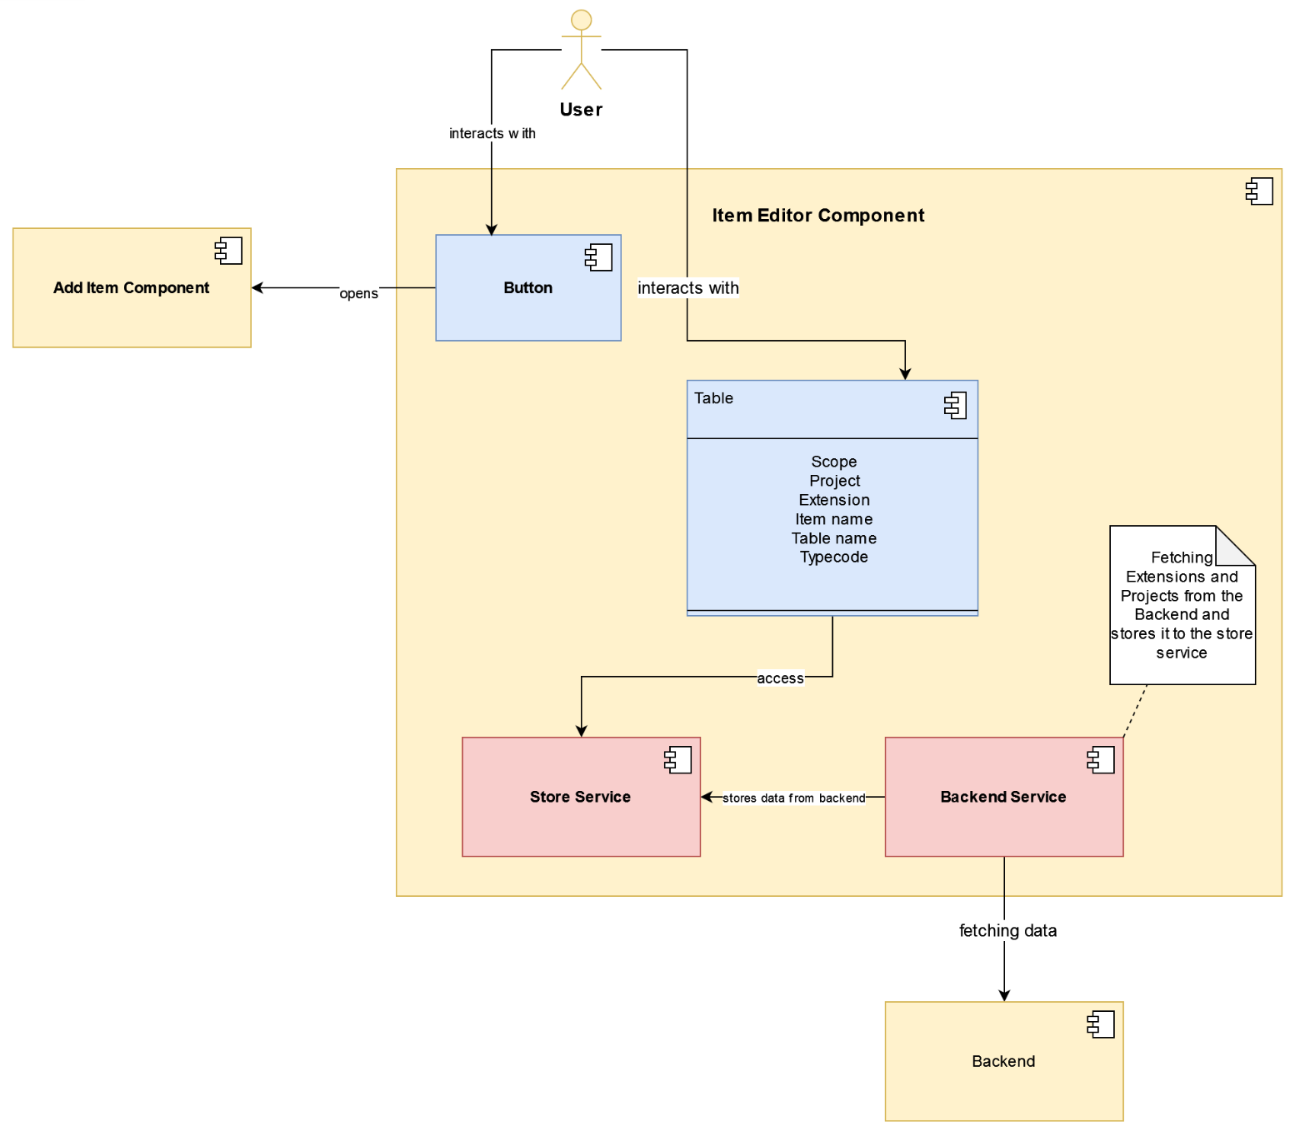
\includegraphics[width=\textwidth]{./images/frontend/item-editor-component}
    \caption{An Illustration of the ItemEditorComponent.}
    \label{fig:itemeditor_component}
\end{figure}

\headingFive{Add Item Component}

This component demonstrates the interactive nature of the application's frontend, providing fields for item details and dynamically adjusting available input options based on user selections.
It interfaces with services to fetch necessary data for dropdown selections and enforces validation rules to ensure data integrity prior to submission.

Figure~\ref{fig:additem_component} presents a schematic view of the \texttt{AddItemComponent}'s architecture, delineating its form structure, the integration with backend services for data fetching, the logic for dynamic display based on scope selection, and the validation mechanisms that underpin its operation.

\begin{figure}[H]
    \centering
    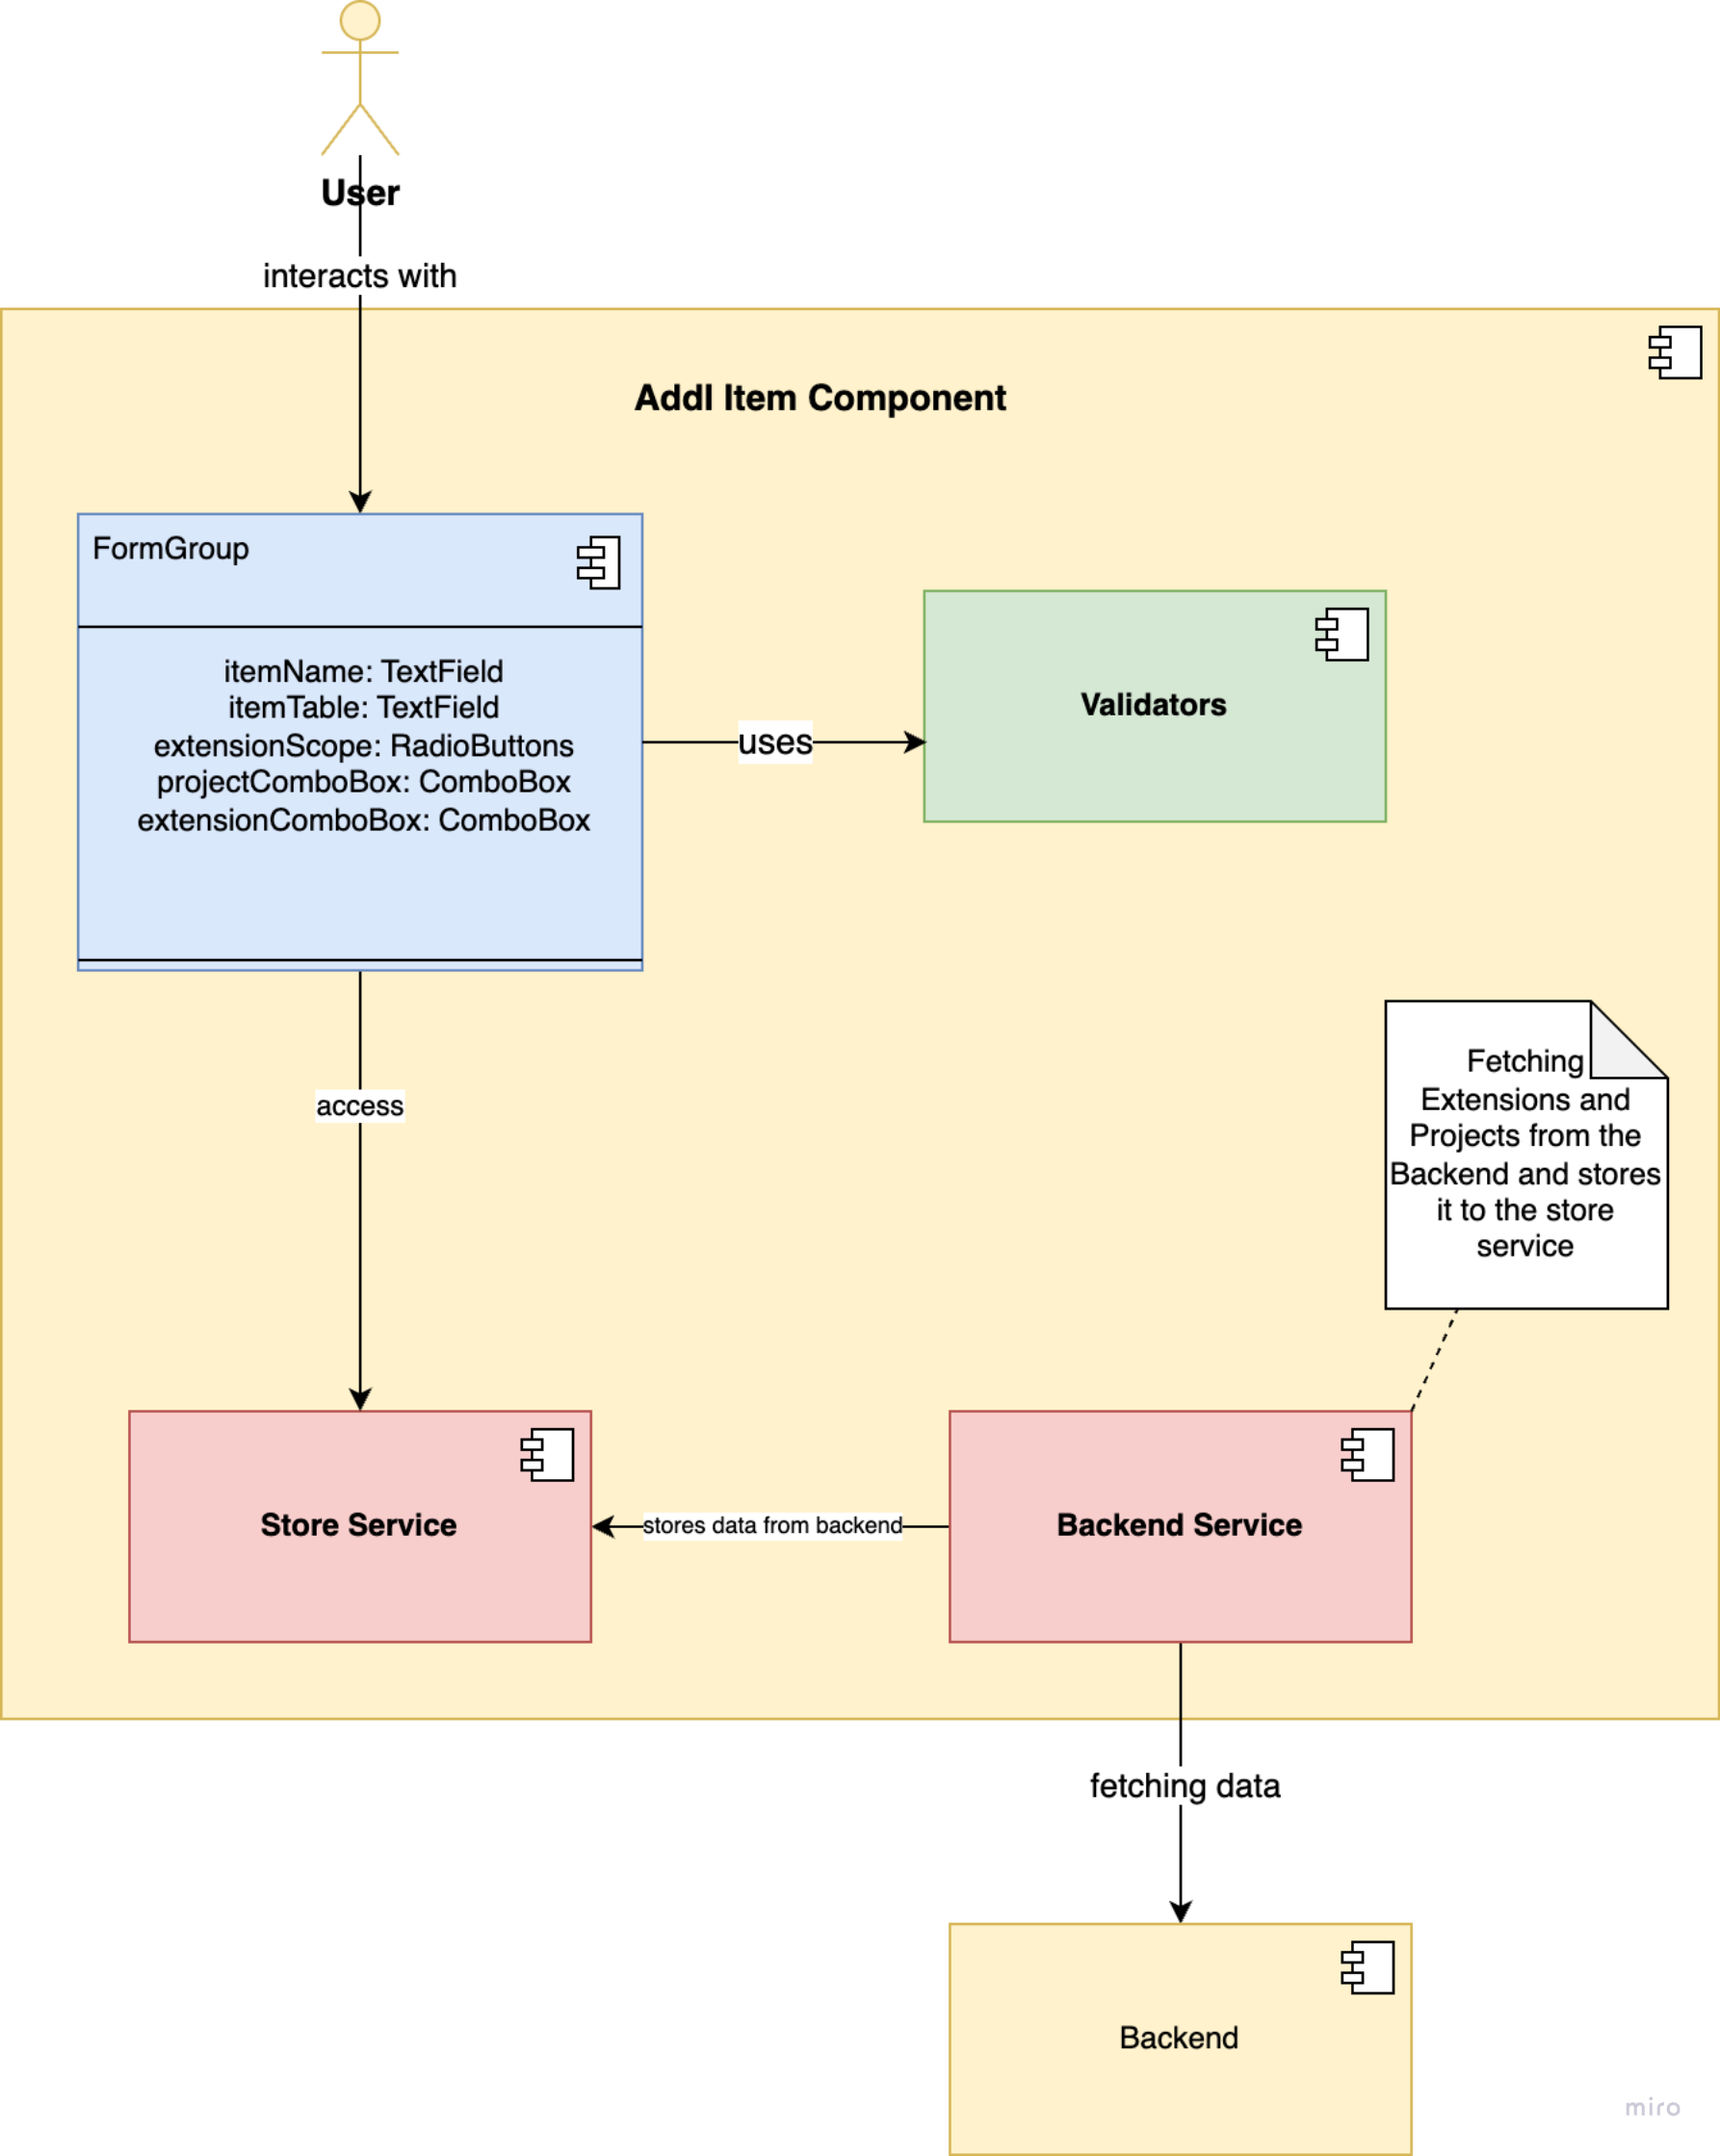
\includegraphics[width=\textwidth]{./images/frontend/add-item-component}
    \caption{The architecture and interaction flow within the AddItemComponent.}
    \label{fig:additem_component}
\end{figure}

\headingSix{Form Structure and User Interaction}
Constructed using Angular's reactive forms, the \texttt{AddItemComponent} orchestrates user interactions through a series of input controls.
Validators attached to these inputs ensure the user-submitted data adheres to the expected formats and business rules.
Upon triggering the submission process, the form data is either emitted to parent components or sent directly to the backend, depending on the configured data flow strategy.

\headingSix{Service Integration}
The component leverages the \texttt{BackendService} to retrieve metadata such as extension types and project scopes.
This data populates the respective form controls, enabling a cohesive and guided user experience.
Through the \texttt{StoreService}, the component accesses a centralized state management pattern, ensuring consistency and reactivity to state changes across the application.

\headingSix{User Input Validation and Error Feedback}
The \texttt{AddItemComponent} is designed with validation functions to ensure that all user inputs meet the necessary criteria before a backend request is initiated to create a new item.
The following fields constitute the user input form:

\begin{itemize}
    \item \textbf{Item Name}: A required field for the name of the item to be created.
    An error message is prompted when the field is not populated upon form submission attempt.
    \item \textbf{Table Name}: A required field specifying the table name for storing item data in SAP. Similar to the item name, it mandates user input to proceed.
    \item \textbf{Scope}: The user must specify the scope—either 'global' or 'project-specific'—for the new item.
    This selection influences the visibility and content of subsequent dropdowns for 'Project' and 'Extension'.
    \item \textbf{Project}: Contingent upon 'Project' scope selection, this mandatory dropdown field allows for the selection of a project from a list populated via the backend.
    \item \textbf{Extension}: This field requires the user to choose an extension from a dynamically loaded dropdown list, based on the selected scope and, if applicable, the selected project.
\end{itemize}

Input validation is enforced by the \texttt{FormGroup}'s built-in validators and custom validator functions such as \texttt{validExtensionValidator} and \\\texttt{validProjectValidator}, which perform checks against the available data retrieved from the \texttt{StoreService}.
The 'Create' button remains inactive as long as any form control remains invalid or unfilled.
The component is structured to prevent form submission if any validation errors persist, ensuring data integrity and user adherence to input requirements.

\headingFive{Update Item Component}

The Update Item Component exemplifies the dynamic and interactive nature of the application's frontend, enabling users to modify existing item details with precision.
It features robust integration with backend services for data retrieval, employs sophisticated user input validation mechanisms, and maintains data integrity throughout the update process.

Figure~\ref{fig:updateitem_component} illustrates the architectural overview of the \texttt{UpdateItemComponent}, delineating its form structure, backend integration for data population, dynamic content adaptation based on user selections, and the validation procedures essential for its operation.

\begin{figure}[H]
    \centering
    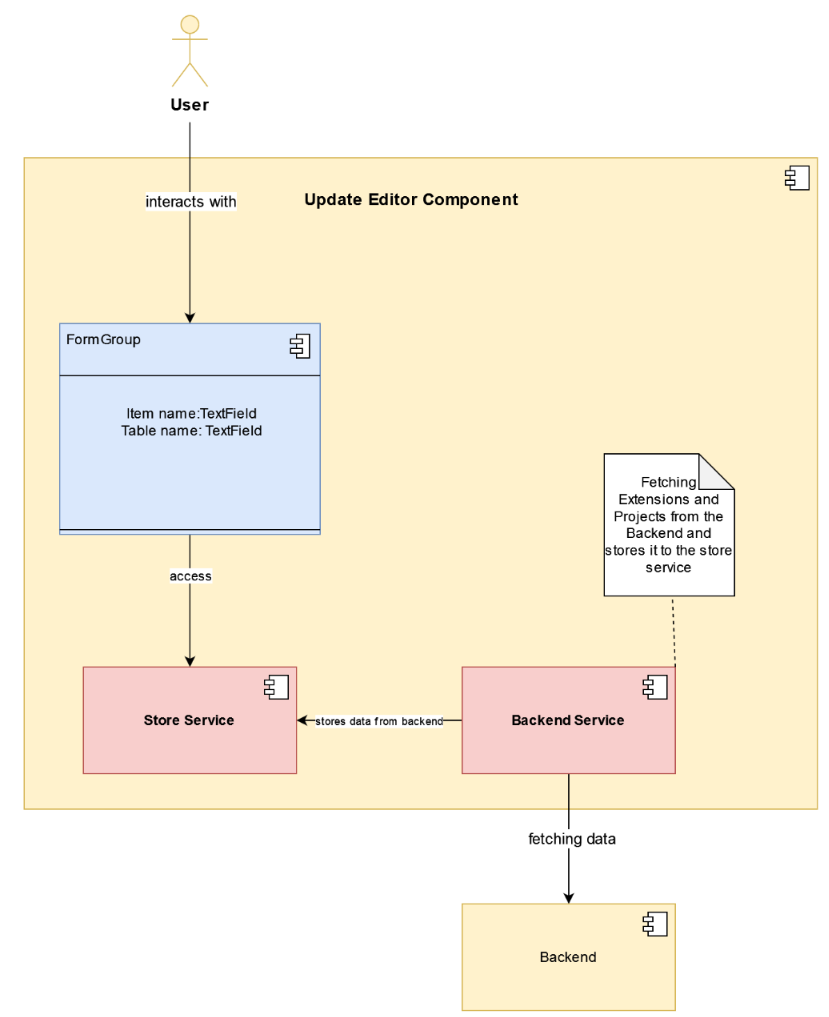
\includegraphics[width=\textwidth]{./images/frontend/update-item-component}
    \caption{Architecture and interaction flow within the UpdateItemComponent.}
    \label{fig:updateitem_component}
\end{figure}

\headingSix{Form Structure and User Interaction}
The Update Item Component is developed using Angular's reactive forms, facilitating seamless user interactions through a series of input controls tailored for modifying item attributes.
Validators are meticulously configured to ensure the accuracy and compliance of user-submitted data with established business rules.
Upon initiating the update process, the modified data is dispatched to the backend for processing or emitted to parent components as dictated by the application's data flow architecture.

\headingSix{Service Integration}
Leveraging the \texttt{BackendService}, the component dynamically retrieves and populates existing item details into the form controls, providing users with contextual information for making informed modifications.
This integration ensures coherence and consistency between the frontend and backend systems.
Additionally, the \texttt{StoreService} is employed to manage the application's state, facilitating real-time updates and maintaining synchronization across various components.

\headingSix{User Input Validation and Error Handling}
The Update Item Component implements robust validation strategies to verify the accuracy and completeness of user inputs before initiating the update operation.
The following key fields constitute the modification form:

\begin{itemize}
    \item \textbf{Item Name}: An essential field for updating the name of the item.
    Input validation prompts an error message if the field is left empty or contains invalid characters.
    \item \textbf{Table Name}: A mandatory field specifying the table name for storing updated item data in SAP. Similar to the item name, user input validation is enforced to ensure data integrity.
\end{itemize}

Validation procedures, including built-in \texttt{FormGroup} validators are employed to verify user selections against available data retrieved from the \texttt{StoreService}.
The 'Update' button remains inactive until all form controls are valid and accurately filled, ensuring adherence to input requirements and safeguarding data consistency during the modification process.

\headingFive{Extension Editor Component}
The \texttt{ExtensionEditorComponent} is a central component that allows users to view, create, update, and delete extensions in the system. It renders a comprehensive table that lists all extensions created, providing users with a quick overview and access to the data they need. The component offers the following functionalities:

\begin{itemize}
    \item \textbf{Display of Data}: The component utilizes a tabular format to present the extension data effectively, allowing for sorting and filtering capabilities to navigate through the extensions conveniently.
    \item \textbf{Interaction with Backend}: It interacts with the backend via the RESTful API to fetch and display the latest extension data.
    \item \textbf{Create New Extensions}: An integral feature of this component is a button that, upon interaction, launches the \texttt{AddExtensionComponent}. This sub-component is a form that captures user input required to create a new extension. When a new extension is created, a success notification is displayed.
    \item \textbf{Delete Extensions}: Users have the ability to delete extensions directly from the displayed list. Upon selecting an extension and triggering the delete action, a confirmation prompt is displayed, and upon confirmation, the extension is removed from the list and deleted from the backend server via the appropriate API endpoint. When a deletion is successful, a success notification is displayed.
    \item \textbf{Update Extensions}: Users can modify existing extensions by selecting an extension from the list and clicking the edit icon.
\end{itemize}

This design ensures that the \texttt{ExtensionEditorComponent} not only serves as a data presentation layer but also as an interactive interface, facilitating the creation and management of extensions.

\begin{figure}[H]
\centering
    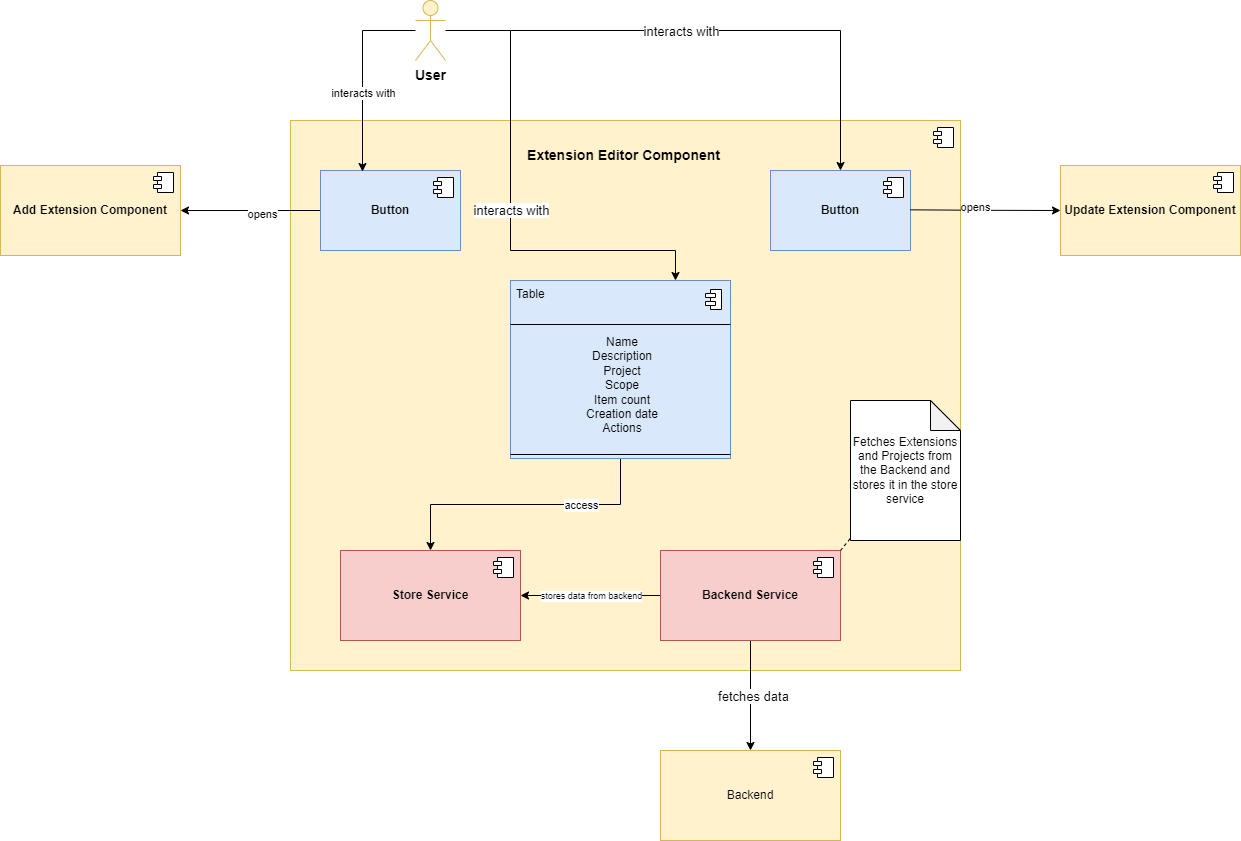
\includegraphics[width=\textwidth]{./images/frontend/extension-editor-component}
    \caption{An Illustration of the ExtensionEditorComponent.}
    \label{fig:extensioneditor_component}
\end{figure}

\headingFive{Add Extension Component}

This component provides fields for extension details and dynamically adjusts the available input options based on user selections.
It interfaces with services to fetch necessary data for dropdown selections and enforces validation rules to ensure data integrity prior to submission.

Figure~\ref{fig:add_extension_component} presents a schematic view of the \texttt{AddExtensionComponent}'s architecture, delineating its form structure, the integration with backend services for data fetching, the logic for dynamic display based on scope selection, and the validation mechanisms that underpin its operation.

\begin{figure}[H]
    \centering
    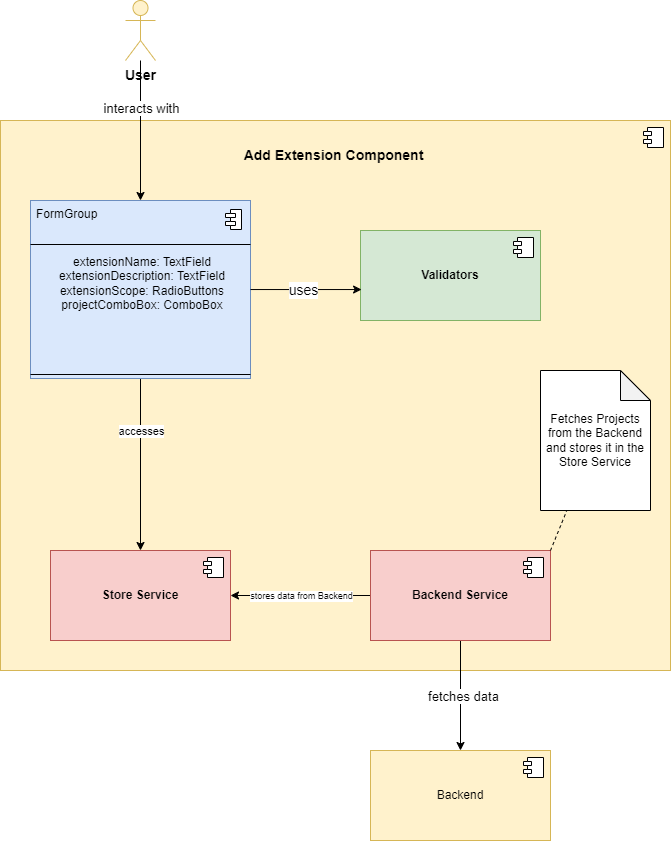
\includegraphics[width=0.95\textwidth]{./images/frontend/add-extension-component}
    \caption{The architecture and interaction flow within the AddExtensionComponent.}
    \label{fig:add_extension_component}
\end{figure}

\headingSix{Form Structure and User Interaction}
Constructed using Angular's reactive forms, the \texttt{AddExtensionComponent} orchestrates user interactions through a series of input controls.
Validators attached to these inputs ensure the user-submitted data adheres to the expected formats and business rules.
Upon triggering the submission process, the form data is either emitted to parent components or sent directly to the backend, depending on the configured data flow strategy.

\headingSix{Service Integration}
The component leverages the \texttt{BackendService} to retrieve metadata such as project names.
This data populates the respective form controls, enabling a cohesive and guided user experience.
Through the \texttt{StoreService}, the component accesses a centralized state management pattern, ensuring consistency and reactivity to state changes across the application.

\headingSix{User Input Validation and Error Feedback}
The \texttt{AddExtensionComponent} is designed with validation functions to ensure that all user inputs meet the necessary criteria before a backend request is initiated to create a new extension.
The following fields constitute the user input form:

\begin{itemize}
    \item \textbf{Extension Name}: A required field for the name of the extension to be created. An error message is prompted when the field is not populated upon form submission attempt.
    \item \textbf{Description}: An optional field where users can enter a description for the extension.
    \item \textbf{Scope of Extension}: The user must specify the scope—either 'Project' or 'Shared'—for the new extension. This selection influences the visibility and content of subsequent dropdowns for 'Project'.
    \item \textbf{Project}: If the 'Project' scope is selected, this mandatory dropdown field allows for the selection of a project from a list populated via the backend.
\end{itemize}

Input validation is enforced by the \texttt{FormGroup}'s built-in validators and custom validator functions such as \texttt{validProjectValidator}, which performs checks against the available data retrieved from the \texttt{StoreService}. The 'Add' button remains inactive as long as any form control remains invalid or unfilled. The component is structured to prevent form submission if any validation errors persist, ensuring data integrity and user adherence to input requirements.

\headingSix{Dynamic Scope Handling}
The component handles scope changes dynamically through the \texttt{scopeChanged} method. This method updates the form's validation state based on the selected scope and ensures the appropriate form controls are validated or cleared as necessary. For instance, when the scope changes from 'Project' to 'Shared', the 'Project' dropdown validators are cleared and the field is reset.

\headingSix{Project Validation}
A custom validator, \texttt{validProjectValidator}, checks the validity of the selected project against the list of projects stored in the \texttt{StoreService}. If the entered project does not exist, a validation error is returned, ensuring that only valid projects can be selected.

\headingFive{Backend Service}
The \texttt{BackendService} acts as the intermediary between the frontend and backend, facilitating data exchange and API calls.
It encapsulates the logic for HTTP requests, error handling, and data transformation, ensuring a seamless communication channel between the Angular application and the Golang backend.

\begin{itemize}
    \item \textbf{HTTP Communication}: Utilizes Angular's HttpClient to make asynchronous HTTP requests to various endpoints, handling CRUD operations with observables that emit data to subscribers upon request completion or error events.
    \item \textbf{Error Handling}: Implements robust error handling mechanisms that capture HTTP errors, transforming them into meaningful messages or actions within the application, thereby enhancing user experience and simplifying debugging efforts.
    \item \textbf{Data Transformation}: Before dispatching the data to calling components, the service processes and transforms the incoming raw data into structured formats defined by TypeScript interfaces, ensuring consistency and type safety across the application.
    \item \textbf{State Management}: Works in tandem with state management solutions, like NgRx or services like \texttt{StoreService}, to maintain application state that is informed by backend responses, enabling reactive UI updates and centralized state handling.
\end{itemize}

The \texttt{BackendService}'s design follows best practices for modern web development, ensuring that the frontend remains decoupled from the backend, promoting maintainability, and allowing the backend to evolve independently with minimal impact on the client-side codebase.

\headingFive{State Management with StoreService}
TODO

\headingFive{Header Component}
The \texttt{HeaderComponent} is a navigational element that provides users with quick access to different sections of the application.
It features a comprehensible menu structure, revealing links to various pages and functionalities within the application.
Those links are:

\begin{itemize}
    \item \textbf{Items (Logo Section)}: Navigates users to the items page of the application.
    \item \textbf{Items}: Directs users to the \texttt{ItemEditorComponent}, where they can view, create, update, and delete items.
    \item \textbf{Projects}: Leads users to a page displaying all projects in the system.
    \item \textbf{Extensions}: Redirects users to the \texttt{ExtensionEditorComponent}, which lists all extensions based on their scope.
    \item \textbf{Settings}: Provides access to user settings.
    \item \textbf{Logout}: Logs users out of the application, terminating the current session.
\end{itemize}

The \texttt{HeaderComponent} is designed to enhance user navigation and streamline access to key features, ensuring a user-friendly and intuitive experience.

\headingFive{Error Display Component}

The \texttt{ErrorDisplayComponent} is responsible for the presentation of custom error pages in response to specific server status scenarios including 204 No Content, 404 Not Found, 500 Internal Server Error, and 520 Unknown Error.
The purpose of this component is to provide users with clear, informative feedback when encountering errors, guiding them on how to proceed or resolve the issue.

\begin{itemize}
    \item \textbf{Error Detection}: Classifying errors based on HTTP status codes.
    \item \textbf{Error Handling}: Displaying a custom error page tailored to the specific error, enhancing the user's understanding of the issue.
    \item \textbf{User Guidance}: Providing actionable advice or options to users for each error scenario, improving user experience during failures.
    \item \textbf{Navigation}: Offering links or buttons to navigate users back to the application's main pages or relevant sections.
\end{itemize}

In all but one case, error codes are sent from the backend to the frontend as part of the HTTP response. The \texttt{ErrorDisplayComponent} interprets those codes and displays the appropriate error description and guidance to the user.
The one exception is the 204 No Content status, which is handled directly by the frontend when no data (null) is received. In case the error is not recognized, a generic error code 520 (Unknown Error) is displayed.
The following table provides an overview of common error scenarios and their corresponding HTTP status codes:

\begin{itemize}
    \item \textbf{0 No Connection}: Suggests that there is no connection to the server, possibly due to network issues or the server being down.
    \item \textbf{204 No Content}: Indicates that the server successfully processed the request but did not return any content owing to the absence of data.
    \item \textbf{404 Not Found}: Signifies that the requested resource could not be found on the server, typically due to an incorrect URL or a missing resource.
    \item \textbf{500 Internal Server Error}: The server encountered an unexpected condition that prevented it from fulfilling the request, often due to a server malfunction. This error may also occur when there is no connection to the database.
    \item \textbf{520 Unknown Error}: This error signifies an unforeseen issue that does not fit into any other category, indicating an ambiguous problem on the server side. It is used as a catch-all for unclassified errors.
\end{itemize}
